\documentclass[compress]{beamer} % no animations

\usepackage{etex} % necessary for pgfplots

\usetheme{AGH}

\graphicspath{{C:/Users/Fysek/Downloads/STiC-slides/figures/}}
\hypersetup{colorlinks, pdfstartview=FitH, bookmarksopen, pdfpagemode=UseNone, pdfpagemode=UseOutlines, linkcolor=black, citecolor=black, filecolor=black, urlcolor=black, pdfauthor={Mateusz Dyrdol}}

% Not all of the following packages are necessary, but the teacher uses many of them :)
% \usepackage{algorithm}
% \usepackage{algpseudocode}
% \usepackage{amsmath,amsfonts}
% \usepackage{amssymb}
% \usepackage{array,supertabular}
\usepackage{bibentry}
% \usepackage{bm}
\usepackage{booktabs}
% \usepackage{cases}
\usepackage{cite}
\usepackage{color}
\definecolor{gold}{HTML}{E6B800}
\definecolor{lightgreen}{HTML}{99CC00}
\definecolor{blue}{HTML}{4D94DB}
\usepackage{colortbl}
\usepackage{comment}
% \usepackage{dsfont}
\usepackage{enumerate}
\usepackage{exscale,relsize}
\usepackage{floatflt}
\usepackage[OT4]{fontenc}
\usepackage{graphicx}
\usepackage[utf8]{inputenc}
\usepackage[utf8]{luainputenc}
% \usepackage{longtable}
% \usepackage{marvosym}
% \usepackage{multirow}
\usepackage{nicefrac}
\usepackage{paralist}
\usepackage{rotating}
\usepackage[tight,footnotesize]{subfigure}
\usepackage{tabularx}
\usepackage{tabulary}
\usepackage{tikz}
\usetikzlibrary{arrows}
\usetikzlibrary{automata}
\usetikzlibrary{backgrounds}
\usetikzlibrary{calc}
\usetikzlibrary{decorations.pathreplacing}
\usetikzlibrary{decorations.pathmorphing}
\usetikzlibrary{fit}
\usetikzlibrary{matrix}
\usetikzlibrary{mindmap}
\usetikzlibrary{patterns}
\usetikzlibrary{petri}
\usetikzlibrary{positioning}
\usetikzlibrary{plothandlers}
\usetikzlibrary{plotmarks}
\usetikzlibrary{shadings}
\usetikzlibrary{shadows}
\usetikzlibrary{shapes}
\usetikzlibrary{shapes.gates.logic.US}
\usetikzlibrary{topaths}
\usetikzlibrary{trees}
\usepackage{pgfplots} % needs \usepackage{etex} just after \documentclass
\pgfplotsset{tick scale binop=\times}
\usepackage{simpsons}
\usepackage{trfsigns}
\usepackage{url}
\usepackage{wasysym}
\usepackage{wrapfig}

\setbeamertemplate{footline}[text line]{
    \leavevmode
    \hbox{
        \begin{beamercolorbox}[wd=\paperwidth,ht=0.01ex,dp=0ex,leftskip=0.25cm,rightskip=0cm plus1fil]{title in head/foot}
            \usebeamerfont{title in head/foot}\logosinfootline
        \end{beamercolorbox}
    }
}\setbeamertemplate{frametitle continuation}[from second][\insertcontinuationtext]

\setbeamercovered{dynamic}
\definecolor{lightgreen}{RGB}{218,238,225}
\setbeamercolor{rafi}{fg=lightgreen,bg=}

\newenvironment{changemargin}[2]{%
    \begin{list}{}{%
        \setlength{\topsep}{0pt}%
        \setlength{\leftmargin}{#1}%
        \setlength{\rightmargin}{#2}%
        \setlength{\listparindent}{\parindent}%
        \setlength{\itemindent}{\parindent}%
        \setlength{\parsep}{\parskip}%
    }%
    \item[]}
{\end{list}}

% \bstctlcite
\makeatletter
    \def\bstctlcite#1{\@bsphack
    \@for\@citeb:=#1\do{%
    \edef\@citeb{\expandafter\@firstofone\@citeb}%
    \if@filesw\immediate\write\@auxout{\string\citation{\@citeb}}\fi}%
    \@esphack}
\makeatother

\newtheorem{remark}{Remark}[theorem]

\abovedisplayshortskip=0pt

\DeclareMathOperator*{\argmin}{arg\,min}

\DeclareMathOperator*{\erf}{erf}

\DeclareMathOperator*{\rank}{rank}

\DeclareMathOperator*{\Dom}{Dom}

\DeclareMathOperator*{\opt}{opt}

\DeclareMathOperator*{\conv}{conv}

\DeclareMathOperator*{\diff}{\!\text{d}}

\DeclareMathOperator*{\mean}{\text{E}}

\DeclareMathOperator*{\logistic}{\text{logistic}}

\newcommand{\eqdef}{%
      \ensuremath{%
          \stackrel{\text{def}}{=}%
      }%
  }

\title{Selected Topics in Cryptography}
\subtitle{Advanced Encryption Standard} 
\author[]{Mateusz Dyrdol} 
\institute[KT AGH]{Department of Telecommunications}
\date{23.10.2017}

\begin{document}

	\begin{frame}
    	\titlepage
	\end{frame}

\setbeamertemplate{background}{
\includegraphics[width=\paperwidth,height=\paperheight]{tlo}}

\renewcommand{\logosinfootline}{\raisebox{0.12cm}{\begin{beamercolorbox}{rafi}{Selected Topics in Cryptography \quad \insertframenumber/\inserttotalframenumber}\end{beamercolorbox}}}
\section{Advanced Encryption Standard} 


\subsection{Agenda}
%%%%%%%%%%%%%%%%%%%%%%%%%%%%%%%%%%%%%%%%%%%%%%%%%%%%%%%%%%%%%%%%%%%%%%%%%%%%%%%%%%%%%%%%%%%%%%%%%%% 
\begin{frame}
	\frametitle{Quantum crypanalysis}
		\framesubtitle{Agenda}
	\vspace{-1cm}
	\hspace{-1.5cm}{	
	\begin{description}
	\item[1.]{Bra-ket notation}
	\item[2.]{Quantum gates}
	\item[3.]{Grover's Database Search}
	\item[4.]{Shore's factorization algorithm}
	\begin{description}
	\hspace{-2.0cm}{• Fast modular exponentiation}\\
	\hspace{-2.0cm}{• Quantum Fourier Transform}\\
	\end{description}
	\end{description}
	}
\end{frame}

%%%%%%%%%%%%%%%%%%%%%%%%%%%%%%%%%%%%%%%%%%%%%%%%%%%%%%%%%%%%%%%%%%%%%%%%%%%%%%%%%%%%%%%%%%%%%%%%%%%	

\subsection{AES Origins}
%%%%%%%%%%%%%%%%%%%%%%%%%%%%%%%%%%%%%%%%%%%%%%%%%%%%%%%%%%%%%%%%%%%%%%%%%%%%%%%%%%%%%%%%%%%%%%%%%%% 
\begin{frame}
	\frametitle{Bra-ket notation}
		\framesubtitle{Origins}
		\vspace{-1cm}
	{\normalsize
	\hspace{0.5cm}{Bra–ket notation: $\braket{x|y}$ is a standard notation for describing quantum states. It can also be used to denote abstract vectors, linear functionals and scalar product in mathematics.}\\
	\vspace{0.4cm}
	\hspace{0.0cm}{The left part: $\bra{x}$, called the bra, is a row vector.}\\
	\hspace{0.0cm}{The right part: $\ket{y}$, called the ket, is a column vector.}\\
	\hspace{0.5cm}{}\\

	}
\end{frame}
%%%%%%%%%%%%%%%%%%%%%%%%%%%%%%%%%%%%%%%%%%%%%%%%%%%%%%%%%%%%%%%%%%%%%%%%%%%%%%%%%%%%%%%%%%%%%%%%%%%

%%%%%%%%%%%%%%%%%%%%%%%%%%%%%%%%%%%%%%%%%%%%%%%%%%%%%%%%%%%%%%%%%%%%%%%%%%%%%%%%%%%%%%%%%%%%%%%%%%% 
\begin{frame}
	\frametitle{Qbit}
		\framesubtitle{Origins}
		\vspace{-1cm}
	{\normalsize
	A pure qubit state is a linear superposition of the basis states. This means that the qubit can be represented as a linear\\ combination of $|0\rangle$ and +$|1\rangle $:\\ 
    $|\psi \rangle =\alpha |0\rangle +\beta |1\rangle$\\
  
    When we measure this qubit in the standard basis, the probability of outcome $|0\rangle$  is $|\alpha |^{2}$ and the probability of outcome $1\rangle$  is $|\beta |^{2}$. Because the absolute squares of the amplitudes equate to probabilities, it follows that
     $\alpha$ and $\beta$ must be constrained by the equation
$$|\alpha |^{2}+|\beta |^{2}=1$$\\
	}
\end{frame}
%%%%%%%%%%%%%%%%%%%%%%%%%%%%%%%%%%%%%%%%%%%%%%%%%%%%%%%%%%%%%%%%%%%%%%%%%%%%%%%%%%%%%%%%%%%%%%%%%%%

%%%%%%%%%%%%%%%%%%%%%%%%%%%%%%%%%%%%%%%%%%%%%%%%%%%%%%%%%%%%%%%%%%%%%%%%%%%%%%%%%%%%%%%%%%%%%%%%%%% 
\begin{frame}
	\frametitle{Gates}
		\framesubtitle{Origins}
		\vspace{-1cm}
	{\normalsize
	\hspace{0.5cm}{In quantum computing and specifically the quantum circuit model of computation, a quantum gate (or quantum logic gate) is a basic quantum circuit operating on a small number of qubits.}\\
	\vspace{0.4cm}
	\hspace{0.5cm}{.}\\
	}
\end{frame}
%%%%%%%%%%%%%%%%%%%%%%%%%%%%%%%%%%%%%%%%%%%%%%%%%%%%%%%%%%%%%%%%%%%%%%%%%%%%%%%%%%%%%%%%%%%%%%%%%%%


\subsection{Grover} 
%%%%%%%%%%%%%%%%%%%%%%%%%%%%%%%%%%%%%%%%%%%%%%%%%%%%%%%%%%%%%%%%%%%%%%%%%%%%%%%%%%%%%%%%%%%%%%%%%%%
\begin{frame}
	\frametitle{Grover's database search}
		\framesubtitle{}

		{\normalsize
		\hspace{0.5cm}{Grover's database search uses possibility to pararell process of qbit. The algorithm allows us to find selected element in unsorted set with complexity $\sqrt{n}$}\\
		}
		

\end{frame}
%%%%%%%%%%%%%%%%%%%%%%%%%%%%%%%%%%%%%%%%%%%%%%%%%%%%%%%%%%%%%%%%%%%%%%%%%%%%%%%%%%%%%%%%%%%%%%%%%%%

%%%%%%%%%%%%%%%%%%%%%%%%%%%%%%%%%%%%%%%%%%%%%%%%%%%%%%%%%%%%%%%%%%%%%%%%%%%%%%%%%%%%%%%%%%%%%%%%%%%
\begin{frame}
	\frametitle{Fast exponentiation}
		\framesubtitle{}

		{\normalsize
		\hspace{0.5cm}{We can calculate $A^{B} mod C$ quickly, using modular multiplication rules:
$$A ^{2} mod C = (A * A) mod C = ((A mod C) * (A mod C)) mod C$$}\\
		}
		

\end{frame}
%%%%%%%%%%%%%%%%%%%%%%%%%%%%%%%%%%%%%%%%%%%%%%%%%%%%%%%%%%%%%%%%%%%%%%%%%%%%%%%%%%%%%%%%%%%%%%%%%%%



\subsection{AES overwiev} 
%%%%%%%%%%%%%%%%%%%%%%%%%%%%%%%%%%%%%%%%%%%%%%%%%%%%%%%%%%%%%%%%%%%%%%%%%%%%%%%%%%%%%%%%%%%%%%%%%%%
\begin{frame}
	\frametitle{Grover's database search}
		\framesubtitle{}
	\vspace{0.5cm}
		\begin{figure}
		\centering
		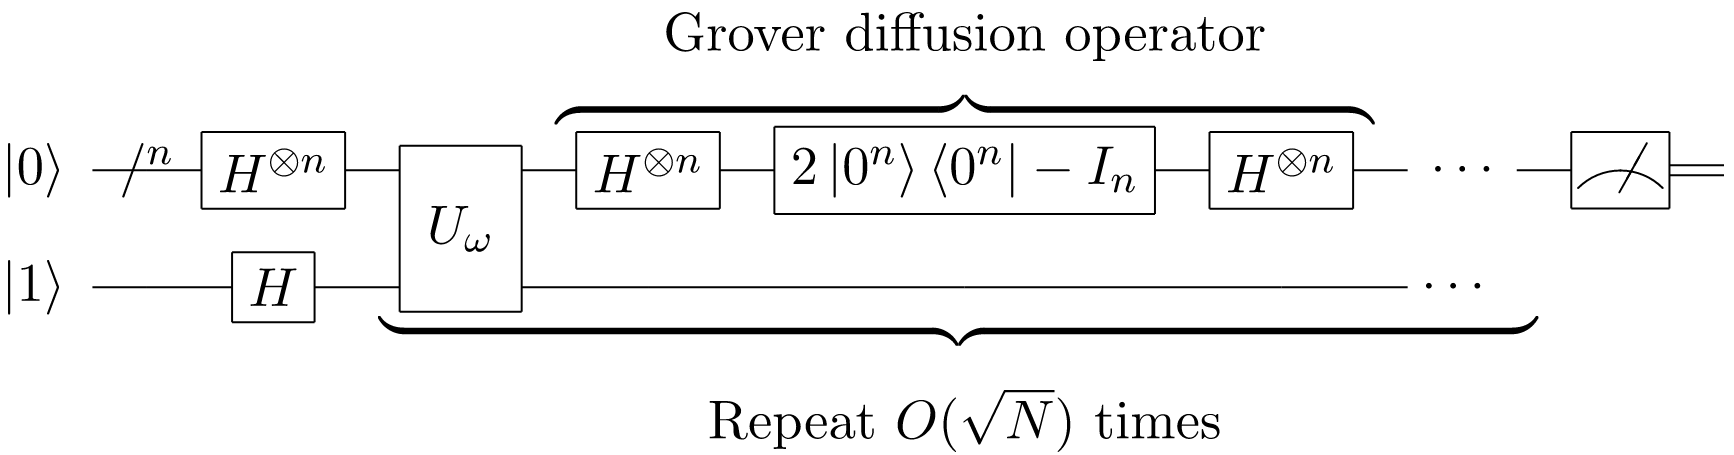
\includegraphics[width=10cm]{grdiffusion}
		\label{fig:grdiffusion grdiffusion}
	\end{figure}
\end{frame}
%%%%%%%%%%%%%%%%%%%%%%%%%%%%%%%%%%%%%%%%%%%%%%%%%%%%%%%%%%%%%%%%%%%%%%%%%%%%%%%%%%%%%%%%%%%%%%%%%%
%%%%%%%%%%%%%%%%%%%%%%%%%%%%%%%%%%%%%%%%%%%%%%%%%%%%%%%%%%%%%%%%%%%%%%%%%%%%%%%%%%%%%%%%%%%%%%%%%%%
\begin{frame}
	\frametitle{Advanced Encryption Standard}
		\framesubtitle{3.MixColumns}
		\vfill
	
	\begin{block}{}
    	{Each column is represented as four-bytes vector.}\\
    \end{block}
    \begin{block}{}
		{Each column of State is replaced by a new column which is formed by multiplying that column by a certain 			matrix of elements of the field.}\\	
	\end{block}	
	    \begin{block}{}
		{Together with ShiftRows, MixColumns provides \textit{diffusion} in the cipher.}\\	
	\end{block}
		\begin{alertblock}{}
		{MixColumns step is used in every cycle \textbf{except} the last one cycle.}\\
		\end{alertblock}
\end{frame}
%%%%%%%%%%%%%%%%%%%%%%%%%%%%%%%%%%%%%%%%%%%%%%%%%%%%%%%%%%%%%%%%%%%%%%%%%%%%%%%%%%%%%%%%%%%%%%%%%%%

%%%%%%%%%%%%%%%%%%%%%%%%%%%%%%%%%%%%%%%%%%%%%%%%%%%%%%%%%%%%%%%%%%%%%%%%%%%%%%%%%%%%%%%%%%%%%%%%%%%
\begin{frame}
	\frametitle{Advanced Encryption Standard}
		\framesubtitle{3.MixColumns }
		
	\begin{block}{}
    	{It is also possible to see this operation as polynomial multiplication where each column is represented with 				 	polynomial a(x):}\\
		\hspace{0.5cm}{$a(x) = c(x).a(x) mod x^{4}+1= ({03}x^3 + {01}x^2 + {01}x + {02})
.(a_3x^3 + a_2x^2 + a_1x^1 + a_0) mod x^4 + 1 $}\\
		
	\end{block}
	\vfill
	\begin{block}{}
	{ $$c(x)= \left[
        \begin{array}{cccc}
         02 & 03\\
         01 & 02
         \end{array}
      \right] $$}
	\end{block}
\end{frame}
%%%%%%%%%%%%%%%%%%%%%%%%%%%%%%%%%%%%%%%%%%%%%%%%%%%%%%%%%%%%%%%%%%%%%%%%%%%%%%%%%%%%%%%%%%%%%%%%%%%

%%%%%%%%%%%%%%%%%%%%%%%%%%%%%%%%%%%%%%%%%%%%%%%%%%%%%%%%%%%%%%%%%%%%%%%%%%%%%%%%%%%%%%%%%%%%%%%%%%%
\begin{frame}
	\frametitle{Advanced Encryption Standard}
		\framesubtitle{Key Schedule: Rcon Table}
		\begin{table}
			\begin{center}
				\setlength\arrayrulewidth{1pt}
				
				\begin{tabular}{|c|c|c|c|}
					\hline 
					\multicolumn{4}{|c|}{Rcon Constants}\\
					\hline
					\hline Round 	& Constant(Rcon)		 &Round  		& Constant(Rcon)		\\
					\hline $1$	 	& $01$ $00$ $00$ $00$    &$6$			&$20$ $00$ $00$ $00$  	\\
					\hline $2$	 	& $02$ $00$ $00$ $00$    &$7$			&$40$ $00$ $00$ $00$  	\\
					\hline $3$	 	& $04$ $00$ $00$ $00$    &$8$			&$80$ $00$ $00$ $00$  	\\
					\hline $4$	 	& $08$ $00$ $00$ $00$    &$9$			&1B $00$ $00$ $00$  	\\
					\hline $5$	 	& $10$ $00$ $00$ $00$    &$10$			&$36$ $00$ $00$ $00$  	\\
					\hline
				\end{tabular}
			\end{center}
		\end{table}

		\vfill
\end{frame}
%%%%%%%%%%%%%%%%%%%%%%%%%%%%%%%%%%%%%%%%%%%%%%%%%%%%%%%%%%%%%%%%%%%%%%%%%%%%%%%%%%%%%%%%%%%%%%%%%%%
 

\subsection{Time for questions}
%%%%%%%%%%%%%%%%%%%%%%%%%%%%%%%%%%%%%%%%%%%%%%%%%%%%%%%%%%%%%%%%%%%%%%%%%%%%%%%%%%%%%%%%%%%%%%%%%%%
\begin{frame}
	
	\begin{center}
		\Huge \textbf{Time for questions}
	\end{center}

\end{frame}
%%%%%%%%%%%%%%%%%%%%%%%%%%%%%%%%%%%%%%%%%%%%%%%%%%%%%%%%%%%%%%%%%%%%%%%%%%%%%%%%%%%%%%%%%%%%%%%%%%%
\subsection{Bibliography}
%%%%%%%%%%%%%%%%%%%%%%%%%%%%%%%%%%%%%%%%%%%%%%%%%%%%%%%%%%%%%%%%%%%%%%%%%%%%%%%%%%%%%%%%%%%%%%%%%%%
\begin{frame}
	\frametitle{Advanced Encryption Standard}
		\framesubtitle{Bibliography}
	{\normalsize 
	
	Bibliography:\\	
	\vspace{0,2cm}
{- Joan Daemen, Vincent Rijmen, "The Design of Rijndael: AES – The Advanced Encryption Standard", Springer, 2002.}\\
\vspace{0,2cm}
{- Joshua Holden, "The Mathematics of Cryptography", Princeton University Press, 2017}\\
\vspace{0,2cm}
{- Federal Information Processing Standards Publication 197 : the official AES standard, United States National Institute of Standards and Technology, 2001}\\
\vspace{0,2cm}
{- Wikipedia, Advanced Encryption Standard, https://en.wikipedia.org/wiki/Advanced$\_$Encryption$\_$Standard}\\

	}
\end{frame}
%%%%%%%%%%%%%%%%%%%%%%%%%%%%%%%%%%%%%%%%%%%%%%%%%%%%%%%%%%%%%%%%%%%%%%%%%%%%%%%%%%%%%%%%%%%%%%%%%%%

\subsection{End}
%%%%%%%%%%%%%%%%%%%%%%%%%%%%%%%%%%%%%%%%%%%%%%%%%%%%%%%%%%%%%%%%%%%%%%%%%%%%%%%%%%%%%%%%%%%%%%%%%%%
\begin{frame}
	
	\begin{center}
		\Huge \textbf{Thank you for attention!}
	\end{center}

\end{frame}
%%%%%%%%%%%%%%%%%%%%%%%%%%%%%%%%%%%%%%%%%%%%%%%%%%%%%%%%%%%%%%%%%%%%%%%%%%%%%%%%%%%%%%%%%%%%%%%%%%% 
\bibliographystyle{plain}
%\nobibliography{bibliographyfile} % your bibliography file

\end{document}